\chapter{Контрмера против атаки с навязыванием ключа} \label{ch:ch3}

%%%%%%%%%%%%%%%%%%%%%%%%%%%%%%%%%%%%%%%%%%%%%%%%%%%%%%%%%%%%%%%%%%%%%%%%%%%%%%%%%%%%%%%%%%%%%%%%%%%%%%%%%%%%%%%%%

\section{Атака с навязыванием ключа «поддельными» состояниями в системе квантовой коммуникации на боковых частотах} \label{sec:ch3/sec1}

В данной главе предлагается реализация атаки с <<поддельными>> состояниями на систему квантовой коммуникации на боковых частотах с используемым в приемном блоке детектором фотонов ID210. Как показали результаты исследования, изложенные во \ref{ch:ch2} главе, этот детектор подвержен выведению из режима Гейгера. Для осуществления успешной атаки между блоками легитимных отправителя и получателя располагается нелегитимный пользователь с аналогичным оборудованием. Всегда при рассмотрении возможностей злоумышленника предполагается, что они ограничены здравым смыслом и законами физики. Таким образом, принципиальная оптическая схема предлагаемой атаки представлена на рисунке \ref{fig:SCW_FSA}. 

 \begin{figure}[ht]
  \centering
  \includegraphics[scale=0.35]{images/scw-setup_FSA_rus1.pdf}
  \caption{Принципиальная оптическая схема предлагаемой атаки с <<поддельными состояниями>>}
  \label{fig:SCW_FSA}
\end{figure}

В состав подсистемы злоумышленника включена приёмная сторона, аналогичная получателю, и модифицированный под атаку блок отправителя. Первая часть подсистемы регистрирует срабатывания в соотвествии с протоколом. Применяемые квантовые состояния, которые привели к конструктивной интерференции, то есть за вычетом ошибок являются аналогичными по отношению к легитимному отправителю передаются в модифицированный блок отправителя. Модификация заключается в том, что в соотвествии с определёнными во \ref{ch:ch2} главе величинами, необходимыми для выведения детектора фотонов из режима Гейгера, источник формирует при помощи лазерного источника высокоинтенсивную несущую, затем в результате фазовой модуляции в спектре формируются боковые частоты, величина которых зависит от индекса модуляции. Весь спектр отправляется в приёмный блок, где в штатном режиме происходит повторная модуляция и интерференция сигналов на боковых частотах в зависимости от применяемых фазовых состояний. Затем отфильтровывается несущая частота, а боковые поступают на детектор одиночных фотонов. При этом мощность сигнала на боковых подбирается таким образом, чтобы её было достаточно для <<ослепления>> детектора и получения срабатывания в те моменты времени, когда злоумышленник отправляет известное, то есть совпавшее с легитимным отправителем, состояние. 


%%%%%%%%%%%%%%%%%%%%%%%%%%%%%%%%%%%%%%%%%%%%%%%%%%%%%%%%%%%%%%%%%%%%%%%%%%%%%%%%%%%%%%%%%%%%%%%%%%%%%%%%%%%%%%%%%
\section{Границы применимости атаки с навязыванием ключа} \label{sec:ch3/sec2}

Разберемся, чем обусловлены и ограничиваются параметры, которые модифицированная подсистема отправителя со стороны злоумышленника должна применять, чтобы успешно проводить предложенную атаку. 

В результате интерференции по аналогии со штатным режимом работы системы квантовой коммуникации с протоколом BB84 возможны 4 исхода, которые схематически представлены на рисунке \ref{fig:Palways}. Если разность фаз, применяемых при фазовой модуляции на стороне отправителя и получателя равна нулю, то интерференция конструктивна(КИ - <<конструктивная интерференция>>), то есть наблюдается усиление сигнала (при равных амплитудах  до четырехкратного увеличения). Если разность фаз равна $\pi$, то интерференция деструктивна (ДИ - <<деструктивная интерференция>>), то есть сигнал ослабляется до минимального уровня (шумов). Если используемые базисы не совпадают (НБ - <<несовпадение базисов>>), то разность фаз в обоих случаях равна $\pi/2$ и наблюдается половинный от максимального, соответствующего КИ, уровень мощности в классическом режиме, либо вероятность срабатывания 0,5 в квантовом режиме. 


 \begin{figure}[ht]
  \centering
  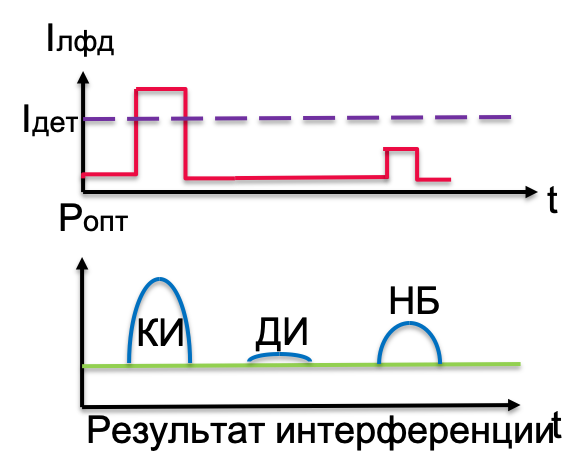
\includegraphics{Palways.png}
  \caption{Методика определения границ применимости}
  \label{fig:Palways}
\end{figure}


Стратегия злоумышленника максимально эффективна в том случае, когда легитимный пользователь с приёмником регистрирует срабатывания только в том случае, когда совпадение у отправителя и приёмной стороны злоумышленника было зафиксировано, а во все остальные моменты должно наблюдаться отсутствие срабатываний. Это условие будет автоматически выполняться в том случае, если фазовое состояние применяемое на приёмной стороне будет в противофазе с состоянием, пришедшим от модифицированной подсистемы злоумышленника, то есть будет наблюдаться ДИ. 

Однако, вариант с несовпадением базисов требует более внимательного рассмотрения. Для выполнения поставленного выше условия в случае несовпадения базисов требуется подобрать мощность контролирующих импульсов так, чтобы в результате интерференции порог срабатывания компаратора по току, протекающему в лавинном фотодиоде, не превысил уровень срабатывания, соответствущий току, необходимому для формирования импульса срабатывания. Это схематически представлено на рисунке \ref{fig:Palways}. Таким образом, накладывается ограничение сверху и снизу на оптическую мощность для контролирующих импульсов. Чтобы приёмный блок не формировал срабатывания, не следует превышать величину оптической мощности $P_\text{никогда}$. Чтобы приёмный блок формировал состояния с единичной вероятностью, следует использовать мощность контролирующих оптических импульсов в пределах от $P_\text{никогда}$ до $P_\text{всегда\_предельное}$, которое равно удвоенному $P_\text{никогда}$:


\[
    \begin{cases}
     P < 2 \cdot P_\text{никогда} \\
     P \geqslant P_\text{всегда}
    \end{cases}
\]




Таким образом, детектор формирует импульс срабатывания только в случае совпадения используемых фазовых состояний, то есть конструктивной интерференции, и не должен формировать этот импульс при несовпадении базисов и деструктивной интерференции. Благодаря этому злоумышленник знает всю информацию о ключе, формируемом легитимными пользователями, а атака получила альтернативное название - <<навязывание ключа>>. Для разных оптических мощностей <<ослепления>> детектора фотонов определены границы применимости использования оптических мощностей контролирующих импульсов для формирования срабатывания и отсутствия срабатывания (рис. \ref{fig:Bounds}).  


 \begin{figure}[ht]
  \centering
  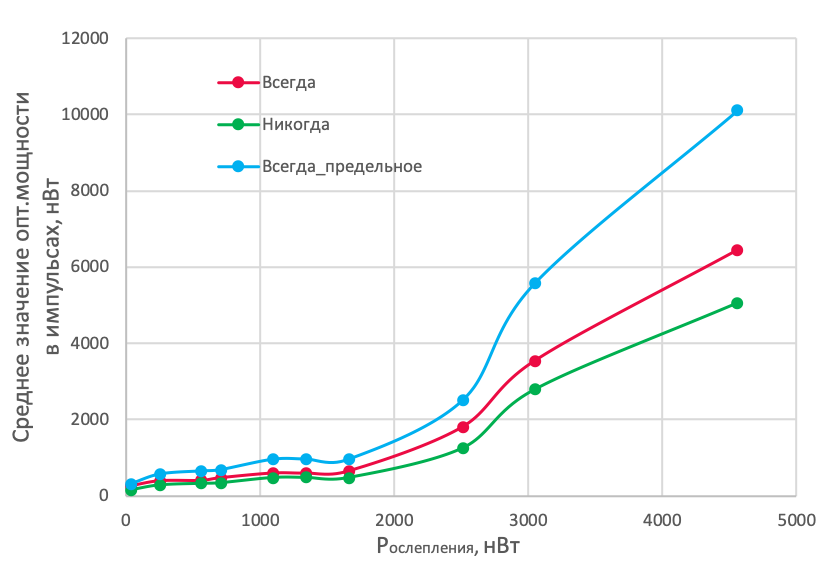
\includegraphics{Bounds.png}
  \caption{Границы применимости используемых оптических мощностей контролирующего импульса и засветки детектора}
  \label{fig:Bounds}
\end{figure}

\pagebreak

%%%%%%%%%%%%%%%%%%%%%%%%%%%%%%%%%%%%%%%%%%%%%%%%%%%%%%%%%%%%%%%%%%%%%%%%%%%%%%%%%%%%%%%%%%%%%%%%%%%%%%%%%%%%%%%%%
\section{Оценка возможностей злоумышленника при атаке с выведением детектора из режима Гейгера для систем квантовой коммуникации на боковых частотах} \label{sec:ch3/sec3}
 
 
 \begin{figure}[ht]
  \centering
  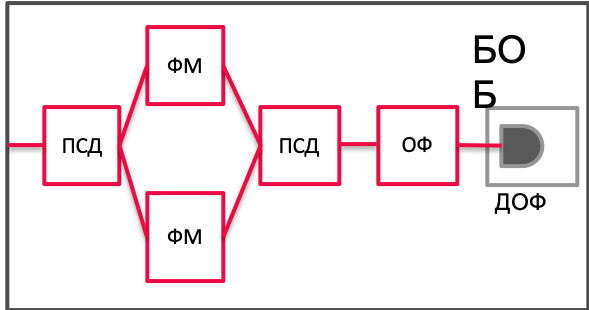
\includegraphics{Bob_scheme1.png}
  \caption{Принципиальная оптическая приемного модуля}
  \label{fig:Bob}
\end{figure}


\begin{table}
	\caption{\label{tab:blinding}Расчетные параметры для контроля детектора в системе квантовой коммуникации на боковых частотах.}
	\begin{tabular}[t]{c c c c}
	\hline\hline
	\makecell{Поддельное\\состояние\\злоумышленника\\мощность в...} & \makecell{Мощность для\\<<ослепления>> (нВт)} & $E_\text{всегда}$ (фДж) & $E_\text{никогда}$ (фДж) \\
	\hline
	\makecell{боковых после\\ фильтрации} & 35 & 25.8 & 15.4 \\
	\makecell{спектре перед\\ модуляцией} & 700 & 516 & 308 \\
	\makecell{спектре на входе\\ в приемный модуль} & 3056 & 2252 & 1345 \\
	\hline\hline
	\end{tabular}
\end{table}


\pagebreak

%%%%%%%%%%%%%%%%%%%%%%%%%%%%%%%%%%%%%%%%%%%%%%%%%%%%%%%%%%%%%%%%%%%%%%%%%%%%%%%%%%%%%%%%%%%%%%%%%%%%%%%%%%%%%%%%%

\section{Оптическая схема для противодействия атаке с <<ослеплением>> ДОФ} \label{ch:ch3/sec4}


 \begin{figure}[ht]
  \centering
  \includegraphics[scale=0.35]{images/scw-setup Countermeasure.pdf}
  \caption{Принципиальная оптическая схема предлагаемой контрмеры против атаки с <<поддельными>> состояниями}
  \label{fig:countermeasure}
\end{figure}

\pagebreak

%%%%%%%%%%%%%%%%%%%%%%%%%%%%%%%%%%%%%%%%%%%%%%%%%%%%%%%%%%%%%%%%%%%%%%%%%%%%%%%%%%%%%%%%%%%%%%%%%%%%%%%%%%%%%%%%%
\section{Экспериментальная проверка контрмеры} \label{ch:ch3/sec5}


 \begin{figure}[ht]
  \centering
  \includegraphics{images/Experimental Countermeasure.pdf}
  \caption{Принципиальная оптическая схема предлагаемой контрмеры против атаки с <<поддельными>> состояниями}
  \label{fig:Experimental_countermeasure}
\end{figure}


\pagebreak
%%%%%%%%%%%%%%%%%%%%%%%%%%%%%%%%%%%%%%%%%%%%%%%%%%%%%%%%%%%%%%%%%%%%%%%%%%%%%%%%%%%%%%%%%%%%%%%%%%%%%%%%%%%%%%%%%
\section{Динамика оптической мощности на мониторном фотодиоде}



\[
    \begin{cases}
     P < 2 \cdot P_\text{никогда} \\
     P \geqslant P_\text{всегда}
    \end{cases}
\]

 \begin{figure}[ht]
  \centering
  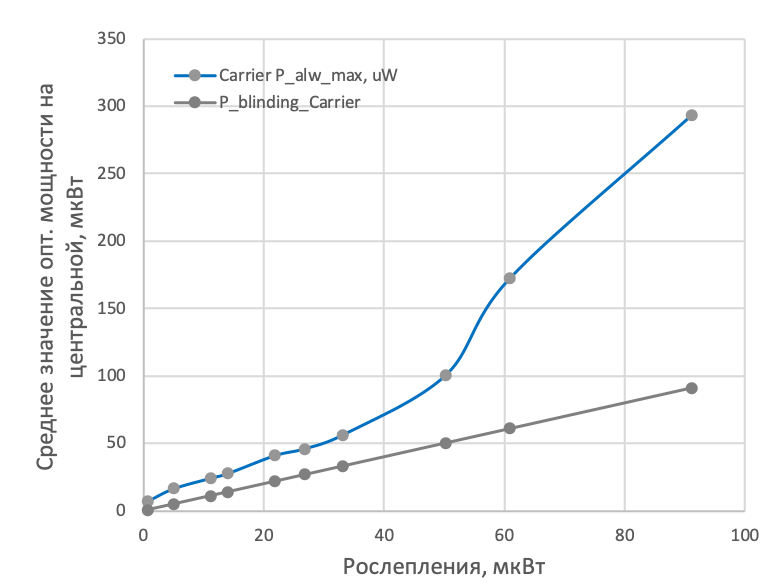
\includegraphics{images/Watchdog_photodiode.png}
  \caption{Динамика и границы оптической мощности на мониторном фотодиоде}
  \label{fig:Watchdog_photodiode}
\end{figure}


\pagebreak
%%%%%%%%%%%%%%%%%%%%%%%%%%%%%%%%%%%%%%%%%%%%%%%%%%%%%%%%%%%%%%%%%%%%%%%%%%%%%%%%%%%%%%%%%%%%%%%%%%%%%%%%%%%%%%%%%
\section{Выводы по главе} \label{ch:ch3/sect7}


В \ref{ch:ch3} главе показано, что измерение величины оптического излучения на несущей частоте, отраженного от оптического фильтра, при помощи мониторного фотодиода в приемном блоке системы квантовой коммуникации на боковых частотах в диапазоне от 7 нВт до 2,93 мкВт с применением дополнительных мер в виде пассивного оптического аттенюатора номиналом 10 дБ для его защиты позволяет противостоять атаке с выведением детектора одиночных фотонов из режима Гейгера и навязыванием ключа нелегитимным пользователем. 
  